\documentclass[journal,onecolumn]{IEEEtran}
\usepackage{amssymb}
\usepackage{graphicx}
\newcommand{\vc}[1]{\mathbf{#1}}


\begin{document}
\title{A Deep Reinforcement Learning Framework for the
	Financial Portfolio Management Problem}


\author{Anıl~Tahmaz,
		Halil~Onur~Fedai,
        and~Muhammed~Mızrak}

%\author{Arash Ashrafnejad}

% make the title area
\maketitle

% As a general rule, do not put math, special symbols or citations
% in the abstract or keywords.
%\begin{abstract}
%Financial portfolio management is the process of constant redistribution of a fund into different financial products. This paper presents a financial-model-free Reinforcement Learning framework to provide a deep machine learning solution to the portfolio management problem. The framework consists of the Ensemble of Identical Independent Evaluators (EIIE) topology, a Portfolio-Vector Memory (PVM), an Online Stochastic Batch Learning
%(OSBL) scheme, and a fully exploiting and explicit reward function. This framework is realized in three instants in this work with a Convolutional Neural Network (CNN), a basic Recurrent Neural Network (RNN), and a Long Short-Term Memory (LSTM). They are, along with a number of recently reviewed or published portfolio-selection strategies, examined in three back-test experiments with a trading period of 30 minutes in a cryptocurrency market.
%Cryptocurrencies are electronic and decentralized alternatives to government-issued money, with Bitcoin as the best-known example of a cryptocurrency. All three instances of the framework monopolize the top three positions in all experiments, outdistancing other
%compared trading algorithms. Although with a high commission rate of 0.25\% in the backtests, the framework is able to achieve at least 4-fold returns in 50 days.
%\end{abstract}



\section{Introduction}
Portfolio management is the decision making process of continuously reallocating an amount of fund into a number of different financial investment products, aiming to maximize the return while restraining the risk \cite{Shapira2009}. Traditional portfolio management methods can be classified into four categories, "Follow-the-Winner", "Follow-the-Loser", "Pattern-Matching", and "Meta-Learning" \cite{Li2014}. The performance of these methods is dependent on the validity of the models on different markets.
There are existing deep machine-learning approaches to financial market trading. However, many of them try to predict price movements or trends \cite{Heaton2017}\cite{Freitas2009}. With history prices of all assets as its input, a neural network can output a predicted vector of asset prices for the next period. Then the trading agent
can act upon this prediction. This idea is straightforward to implement, because it is a supervised learning, or more specifically a regression problem. The performance of these
price-prediction-based algorithms, however, highly depends on the degree of prediction accuracy, but it turns out that future market prices are very difficult to predict. Furthermore, it is difficult for a prediction-based network to consider transaction cost as a risk factor.
Previous successful attempts of model-free and fully machine-learning schemes to the algorithmic trading problem, without predicting future prices, are treating the problem as a Reinforcement Learning (RL) one \cite{Moody2001}\cite{Dempster2006}\cite{Deng2017}. These
RL algorithms output discrete trading signals on an asset. Being limited to single-asset trading, they are not applicable to general portfolio management problems, where trading agents manage multiple assets.


Deep RL is lately drawing much attention due to its remarkable achievements in playing video games and board games \cite{Silver2014}. These are RL
problems with discrete action spaces, and can not be directly applied to portfolio selection problems, where actions are continuous. Although market actions can be discretized, discretization is considered a major drawback, because discrete actions come with unknown risks. In addition, discretization scales badly. In order to take full advantage of adaptability of machine learning over different
markets, trading algorithms have to be scalable.

A general-purpose continuous deep RL framework, the actor-critic Deterministic Policy Gradient Algorithms, was recently introduced \cite{Silver2014}. The continuous output in these actor-critic
algorithms is achieved by a neural-network approximated action policy function, and a second network is trained as the reward function estimator. Training two neural networks,however, is found out to be difficult, and sometimes even unstable.

This paper proposes an RL framework specially designed for the task of portfolio management. The core of the framework is the Ensemble of Identical Independent Evaluators (EIIE) topology. An IIE is a neural network whose job is to inspect the history of an asset and evaluate its potential growth for the immediate future. Apart from the market history, portfolio weights from the previous trading period are also input to the EIIE. This is for the RL agent to consider the effect of transaction cost to its wealth. Being a fully machine-learning approach, the framework is not restricted to any particular markets. To examine its validity and profitability, the framework is tested in a cryptocurrency exchange market, Polonix.com.

Two natures of cryptocurrencies differentiate them from traditional financial assets, making their market the best test-ground for algorithmic portfolio management experiments. These natures are decentralization and openness, and the former implies the latter. Without a central regulating party, anyone can participate in cryptocurrency trading with low entrance requirements. One direct consequence is abundance of small-volume currencies. Affecting the prices of these penny-markets will require smaller amount of investment, compared to traditional markets. This will eventually allow trading machines to learn and take advantage of the impacts by their own market actions. Openness also means the markets are more accessible. 
\section{Problem Definition}
This section provides a mathematical setting of the portfolio
management problem.
\subsection{Trading Period}
In this work, trading algorithms are time-driven, where time is divided into periods of equal
lengths $T$ . At the beginning of each period, the trading agent reallocates the fund among the assets. $T = 30$ minutes in all experiments of this paper. The price of an asset goes up and
down within a period, but four important price points characterize the overall movement of a period, namely the opening, highest, lowest and closing prices. For continuous markets, the opening price of a financial instrument in a period is the closing price from the previous period. It is assumed in the back-test experiments that
at the beginning of each period assets can be bought or sold at the opening price of that period. The justification of such an assumption is given in Hypotheses section.
\subsection{Mathematical Formalism}
The portfolio consists of $m$ assets. The closing prices of all assets form the \textit{price vector} $\vc{v_t}$ for each Period t. Similarly, $v^{(hi)}_t$ and $v^{(lo)}_t$ denote the highest and lowest prices of the period. The first asset in the portfolio is special, that it is the quoted currency, referred to
as the cash for the rest of the article. Therefore the first price elements are always zero, that is $v^{(hi)}_{0,t} = v^{(lo)}_{0,t} = v_{0,t} = 1, \forall t$. In the experiments of this paper, the cash is Bitcoin.

Note that for continuous markets, elements of $\vc{v_t}$ are the opening prices for Period $t + 1$ as well as the closing prices for Period t. The \textit{price relative} vector of the $t$th trading period, $\vc{y_t}$, is defined as the element-wise division of $\vc{y_t}$ by $\vc{y_{t-1}}$:
\begin{equation}
	\vc{y_t}:=\vc{v_t}\oslash\vc{v_{t-1}} = (1, \frac{v_{1,t}}{v_{1,t-1}}, \frac{v_{2,t}}{v_{2,t-1}}, ..., \frac{v_{m,t}}{v_{m,t-1}})^\top
\end{equation}

The price relative vector can be used to calculate the change in total
portfolio value in a period. If $p_{t-1}$ is the portfolio value at the begining of Period t, ignoring transaction cost,

\begin{equation}
	p_t = p_{t-1}\vc{y_t}\cdot\vc{w_{t-1}}
\end{equation}

where $\vc{w_{t-1}}$ is the portfolio weight vector (referred to as the \textit{portfolio vector} from now on) at the beginning of Period t, whose $i$th element, $w_{t-1,i}$, is the proportion of asset i in the portfolio after capital reallocation. Note that, the elements of portfolio vector should sum up to one. Then, the \textit{rate of return} is

\begin{equation}
	\rho_t := \frac{p_t}{p_{t-1}} - 1 = \vc{y_t}\cdot\vc{w_{t-1}} - 1
\end{equation}

and the corresponding \textit{logarithmic rate of return} is
\begin{equation}
r_t := \ln \frac{p_t}{p_{t-1}} = \ln \vc{y_t}\cdot\vc{w_{t-1}}
\end{equation}

If there is no transaction cost, the final portfolio value will be
\begin{equation}
p_f = p_0 \exp (\sum_{t=1}^{t_f+1} r_t) = p_0 \prod_{t=1}^{t_f+1} \vc{y_t}\cdot\vc{w_{t-1}}
\end{equation}
where $p_0$ is the initial investment amount. The objective of a portfolio manager is to maximize $p_f$ for a given time frame $t_f$.


\subsection{Transaction Cost}
In a real-world scenario, buying or selling assets in a market is not free. The cost is normally from commission fee. Assuming a constant commission rate, this section will re-calculate
the final portfolio value in Equation (5), using a recursive formula extending a work by \cite{Ormos2013}.

After every time period, the portfolio manager needs to reallocate the portfolio in order to obtain the next desired portfolio vector $\vc{w_t}$. This reallocation action shrinks the portfolio value by a factor $\mu_t$, $\mu_t \in(0, 1]$, and will be called the \textit{transaction remainder factor} from now on. Therefore, the final portfolio value in Equation (5) becomes





\begin{equation}
p_f = p_0 \prod_{t=1}^{t_f+1} \mu_t \vc{y_t}\cdot\vc{w_{t-1}}
\end{equation}

Finding the transaction remainder factor $\mu_t$ is not a straightforward task and it involves using recursive methods. In general, $\mu_t$ and its approximations are functions of portfolio vectors of two recent periods and the price relative vector,
\begin{equation}
	\mu_t = \mu_t(\vc{w_{t-1}}, \vc{w_{t}}, \vc{y_{t}}).
\end{equation}
Throughout this work, a single constant commission rate for both selling and purchasing for all non-cash assets is used, $c_s = c_p = 0.25\%$, which is the maximum rate at Poloniex Exchange.

The author of the study in-\cite{Jiang2017} is shown that $\mu_t$ is governed by the following equation,

\begin{equation}
	\mu_t = \frac{1}{1-c_pw_{t,0}}[1-c_p w_{t,0}' - (c_s+c_p-c_s c_p)\sum_{i=1}^{m}(w_{t,i}'-\mu_t w_{t,i})^+ ]
\end{equation}

where $\vc{w_t'}$ is defined as follows,
\begin{equation}
\vc{w_t'}= \frac{\vc{y_t \odot \vc{w_{t-1}}}}{\vc{y_t \cdot \vc{w_{t-1}}}}
\end{equation}

Note that The presence of $\mu_t$ inside a linear rectifier means $\mu_t$ is not analytically solvable, but it can be solved iteratively.

The paper is further proved that there is a sequence $\{\tilde{\mu}_t^{(k)}\}$ that converges to $\mu_t$ and is defined as,

\begin{equation}
	\{\tilde{\mu}_t^{(k)} | \tilde{\mu}_t^{(0)} = \mu_{\odot}  \quad and \quad \tilde{\mu}_t^{(k)} = f(\tilde{\mu}_t^{(k-1)}) , k \in \mathbb{N}_0 \}
\end{equation}
where function $f$ is defined from the Equation 8,
\begin{equation}
f(\mu_t) := \frac{1}{1-c_pw_{t,0}}[1-c_p w_{t,0}' - (c_s+c_p-c_s c_p)\sum_{i=1}^{m}(w_{t,i}'-\mu_t w_{t,i})^+ ]
\end{equation}

This theorem provides a way to approximate the transaction remainder
factor $\mu_t$ to an arbitrary accuracy. The speed on the convergence depends on the error of the initial guest $\mu_{\odot}$.
When $c_p = c_s = c$, there is a practice in-\cite{Moody2001} to approximate $\mu_t$ with $c\sum_{i=1}^{m}|w_{t,i}'-w_{t,i}|$. Therefore, in this work, $\mu_{\odot}$ will use this as the first value for the sequence,
that is, 
\begin{equation}
	\mu_{\odot} = c\sum_{i=1}^{m}|w_{t,i}'-w_{t,i}|
\end{equation}

In summary, the purpose of the algorithmic agent is to generate a time-sequence of portfolio vectors $\{\vc{w_1}, \vc{w_2}, · · · , \vc{w_t}, · · · \}$ in order to maximize the accumulative capital in Equation (6), taking transaction cost into account.

\subsection{Two Hypotheses}
In this work, back-test tradings are only considered, where the trading agent pretends to be
back in time at a point in the market history, not knowing any "future" market information,
and does paper trading from then onward. As a requirement for the back-test experiments,
the following two assumptions are imposed:

\begin{enumerate}
	\item Zero slippage: The liquidity of all market assets is high enough that, each trade can
	be carried out immediately at the last price when a order is placed.
	\item Zero market impact: The capital invested by the software trading agent is so insignificant
	that is has no influence on the market.
\end{enumerate}

In a real-world trading environment, if the trading volume in a market is high enough, these two assumptions are near to reality.

\section{Data Treatments}
The trading experiments are done in the exchange Poloniex, where there are about 80 tradable cryptocurrency pairs with about 65 available cryptocurrencies\footnote{as of May 23, 2017.}. However, for the
reasons given below, only a subset of coins is considered by the trading robot in one period.
Apart from coin selection scheme, this section also gives a description of the data structure that the neural networks take as their input, a normalization pre-process, and a scheme to
deal with missing data.

\subsection{Asset Pre-Selection}
In the experiments of the paper, the 11 most-volumed non-cash assets are preselected for the portfolio. Together with the cash, Bitcoin, the size of the portfolio, m + 1, is 12. This number is chosen by experience and can be adjusted in future experiments. For markets with large volumes, like the foreign exchange market, m can be as big as the total number of available assets.
However, using top volumes for coin selection in back-test experiments can give rise to a \textit{survival bias}. The trading volume of an asset is correlated to its popularity, which in turn is governed by its historic performance. Giving future volume rankings to a backtest, will inevitably and indirectly pass future price information to the experiment, causing unreliable positive results. For this reason, volume information just before the beginning of the back-tests is taken for preselection to avoid survival bias.

\subsection{Price Tensor}
The input to the neural networks at the end of Period $t$ is a tensor, $\vc{X_t}$, of rank 3 with shape $(f, n, m)$, where $m$ is the number of preselected non-cash assets, $n = 50$ is the number of
input periods before $t$, and $f = 3$ is the feature number corresponding to closing, highest, and lowest price relative vectors in
the interval.	
\subsection{Filling Missing Data}
Some of the selected coins lack part of the history. This absence of data is due to the fact that these coins just appeared relatively recently. Data points before the existence of a coin are marked as Not A Numbers (NANs) from the exchange.

These NAN prices are replaced by fake constant prices in order to not affect the future decision of the networks.

\section{Reinforcement Learning}
With the problem defined in Section 2 in mind, this section presents a reinforcement learning(RL) solution framework using a deterministic policy gradient algorithm. The explicit reward function is also given under this framework

\subsection{The Environment and the Agent}
In the problem of algorithmic portfolio management, the agent is the software portfolio manager performing trading-actions in the environment of a financial market. This environment comprises of all available assets in the markets and the expectations of all market participants towards them \cite{Jiang2017}.

It is impossible for the agent to get total information of a state of such a large and complex environment. Nonetheless, all relevant information is believed, in the philosophy
of technical traders\cite{Lo2000}, to be reflected in the prices of the assets, which are publicly available to the agent. Under this point of view, an environmental
state can be roughly represented by the prices of all orders throughout the market’s history up to the moment where the state is at. Although full order history is in the public domain for many financial markets, it is too huge a task for the software agent to practically process this information. As a consequence, sub-sampling schemes for the order-history information are employed to further simplify the state representation of the market environment. These
schemes include asset preselection as described before, periodic feature extraction (i.e., taking 30 min interval) and history cut-off (i.e., taking the last 50 periods).

The agent’s buying and selling transactions made at the beginning of Period $t + 1$, aiming to redistribute the wealth among the assets can be determined by $\vc{w_{t-1}}$ and $\vc{w_{t}}$. Since $\vc{w_{t-1}}$ is already determined at the last period, the action of the agent at time $t$ can be represented solely by the portfolio vector $\vc{w_{t}}$,

\begin{equation}
	\vc{a_t} = \vc{w_{t}}
\end{equation}

Therefore, the state at $t$ is represented as the pair of $\vc{X_t}$ and $\vc{w_{t-1}}$,
\begin{equation}
	\vc{s_t} = (\vc{X_t}, \vc{w_{t-1}})
\end{equation}
Because under Hypothesis 2, the portfolio
amount is negligible compared to the total trading volume of the market, $p_t$ is not included in the internal state.

\subsection{Reward Function}
It is the objective of the agent to maximize the final portfolio value $p_f$ of Equation (6) at the
end of the $t_f + 1$ period. As the agent does not have control over the choices of the initial investment, $p_0$ , and the length of the whole portfolio management process, $t_f$, this job is equivalent to maximizing the average logarithmic cumulated return $R$,

\begin{equation}
	R(s_1, a_1,..., s_{t_f} , a_{t_f} , s_{t_f +1} ) := \frac{1}{t_f}ln\frac{p_f}{p_0} = \frac{1}{t_f}\sum_{t=1}^{t_f+1}ln(\mu_t \vc{y_t}\cdot\vc{w_{t-1}})=\frac{1}{t_f}\sum_{t=1}^{t_f+1}r_t
\end{equation}
In the language of RL, $R$ is the cumulated reward, and $r_t /t_f$ is the immediate reward for an individual episode. The denominator $t_f$ guarantees the fairness of the reward function between runs of different lengths, enabling it to train the trading policy in mini-batches.

With this reward function, the current framework has two important distinctions from many other RL problems. One is that both the episodic and cumulated rewards are exactly
expressed. In other words, the domain knowledge of the environment is well-mastered, and can be fully exploited by the agent. This exact expressiveness is based upon Hypothesis
1 that an action has no influence on the external part of future states, the price tensor. This isolation of action and external environment also allows one to use the same segment of market history to evaluate different sequences of actions.

The second distinction is that all episodic rewards are equally important to the final return. This distinction, together with the zero-market-impact assumption, allows $r_t /t_f$ to be regarded as the action-value function of action $\vc{w_t}$ with a discounted factor of 0, taking
no consideration of future influence of the action. This allows to avoid local optima with a full-exploitation approach (no exploration in other RL problems) as discussed in the next section.
\subsection{Deterministic Policy Gradient}
A policy is a mapping from the state space to the action space, $\pi : S \rightarrow A$. With full exploitation in the current framework, an action is deterministically produced by the policy from a state. The optimal policy is obtained using a gradient ascent algorithm. To achieve this, a policy is specified by a set of parameter $\vc{\theta}$, and $\vc{a_t} = \pi_{\vc{\theta}}(\vc{s_t} )$. The performance metric of $\pi_{\vc{\theta}}$ for time interval $[0, t_f ]$ is defined as the corresponding reward function (15) of the interval,
\begin{equation}
	J_{[0,t_f]}(\pi_{\theta})  = R(s_1, a_1,..., s_{t_f} , a_{t_f} , s_{t_f +1} )
\end{equation}
After random initialisation, the parameters are continuously updated along the gradient direction with a learning rate $\lambda$,

\begin{equation}
	\vc{\theta} \rightarrow \vc{\theta}+\lambda \nabla_{\vc{\theta}}J_{[0,t_f]}(\pi_{\theta})
\end{equation}
To improve training efficiency and avoid machine-precision errors, $\vc{\theta}$ will be updated upon mini-batches instead of the whole training market-history. If the time-range of a mini-batch is $[t_{b_1} , t_{b_2}]$, the updating rule for the batch is,
\begin{equation}
\vc{\theta} \rightarrow \vc{\theta}+\lambda \nabla_{\vc{\theta}}J_{[t_{b_1} , t_{b_2}]}(\pi_{\theta})
\end{equation}
This mini-batch approach of gradient ascent also allows online learning, which is important in online trading where new market history keep coming to the agent. Details of the online learning and mini-batch training will be discussed later.
\section{Policy Networks}
The policy functions $\vc{\theta}$ will be constructed using three different deep neural networks.
The three incarnations of neural networks which is tried to build up the policy functions are a CNN, a basic RNN, and a LSTM. Since CNN was the most successful model in the original study we focus our attention to this model here.

\subsection{CNN Network Topology}
A fully convolutional network is used to implement the Ensemble of Identical Independent Evaluators (EIIE) as illustrated in Figure 1. The first dimensions of all the local receptive fields in all feature maps are 1, making all rows isolated from each other until the softmax activation (hence Independent Evaluator). Each row of the entire network is assigned with a particular asset, and is responsible to submit a voting score to the softmax on the growing potential of the asset in the coming trading period. The previous portfolio weights, $\vc{w_{t-1}}$, are inserted as an extra feature map before the scoring layer, for the agent to minimize transaction cost. These streams are like independent but identical networks of smaller scopes, separately observing and assessing individual non-cash assets. They only interconnect at the softmax function, just to make sure their outputting weights are non-negative and summing up to unity. The authors call these streams mini-machines or more formally Identical Independent Evaluators (IIE), and this topology feature Ensemble of IIE (EIIE) is nicknamed mini-machine approach. 

EIIE greatly improves the performance of the portfolio management. Because if remembering the historic performance of individual assets, an integrated network is more reluctant to invest money to a historically unfavorable asset, even if the asset has a much more promising future. On the other hand, without being designed to reveal the identity of the assigned asset, an IIE is able to judge its potential rise and fall merely based on more recent events.

From a practical point of view, EIIE has three other crucial advantages over an integrated network. The first is scalability in asset number. Having the mini-machines all identical with shared parameters, the training time of an ensemble scales roughly linearly with m. The second advantage is data-usage efficiency. For an interval of price history, a mini-machine can be trained m times across different assets. Asset assessing experience of the IIEs is then shared and accumulated in both time and asset dimensions. The final advantage is plasticity to asset collection. Since an IIE’s asset assessing ability is universal without being restricted to any particular asset, an EIIE can update its choice of assets and/or the size of the portfolio in real-time, without having to train the network again from ground zero.

\begin{figure}[!t]
\centering
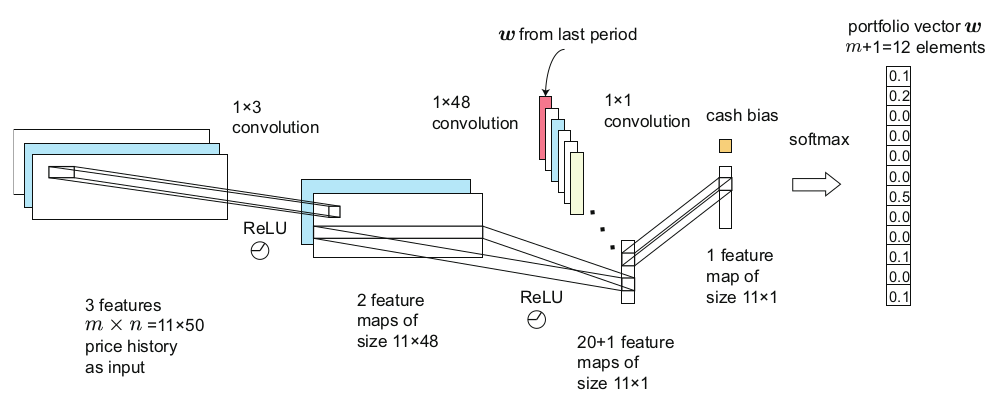
\includegraphics[width=0.8\linewidth]{CNN.png}
\caption{CNN Implementation of the EIIE}
\label{fig_sim}
\end{figure}
\subsection{Portfolio-Vector Memory}
In order for the portfolio management agent to minimize transaction cost by restraining itself from large changes between consecutive portfolio vectors, the output of portfolio weights from the previous trading period is input to the networks.

In this work a dedicated Portfolio-Vector Memory (PVM), is introduced to store the network outputs. Before any network training, the PVM is initialized with uniform weights. In each training step, a policy network loads the portfolio vector of the previous period from the memory location at $t - 1$, and overwrites the memory at $t$ with its output.
\subsection{Online Stochastic Batch Learning}
The ever-ongoing nature of financial markets means new data keeps pouring into the agent, and as a consequence the size of the training sample explodes indefinitely. Fortunately, it is believed that the correlation between two market price events decades exponentially with the temporal distance between them \cite{Holt2004}. With this belief, here an Online Stochastic Batch Learning (OSBL) scheme is proposed.
At the end of the $t$th period, the price movement of this period will be added to the training set. After the agent has completed its orders for period $t + 1$, the policy network will be trained against $N_b$ randomly chosen mini-batches from this set. if the uniform batch size is $n_b$ , data sets covering $[t_b , t_b + n_b )$ is a mini-batch. A batch starting with period $t_b \le t - n_b$ is picked with a geometrically distributed probability $P_{\beta}(t_b)$,

\begin{equation}
	P_{\beta}(t_b) = \beta(1 - \beta)^{t-t_b-n_b}
\end{equation}
where $\beta \in (0, 1)$ is the probability-decaying rate determining the shape of the probability distribution and how important are recent market events, and $n_b$ is the number of periods
in a mini-batch.

\section{Experiments}
The tools has been developed to this point of the article are examined in three back-test experiments of different time frames with all three policy networks on the crypto-currency exchange Poloniex. Results are compared with many well-established and recently published
portfolio-selection strategies. The main compared financial metric is the portfolio value as well as maximum drawdown and the Sharpe ratio. The description of test ranges is omitted here for conciseness since it is shown in the plots.

\subsection{Performance Measures}
Different metrics are used to measure the performance of a particular portfolio selection strategy. The most direct measurement of how successful is a portfolio management over a timespan is the accumulative portfolio value (APV), $p_t$. It is unfair, however, to compare the PVs of two management starting of different initial values. Therefore, APVs here are measured in the unit of their initial values, or equivalently $p_0 = 1$ and under the same unit, the final APV (fAPV) is the APV at the end of a back-test experiment, $p_f = p_f /p_0$.

A major disadvantage of APV is that it does not measure the risk factors, since it merely sums up all the periodic returns without considering fluctuation in these returns. A second metric, the Sharpe ratio (SR) \cite{Sharpe1994} is used to take risk into account. The
ratio is a risk adjusted mean return, defined as the average of the risk-free return by its deviation,

\begin{equation}
	S = \frac{\mathbb{E} [\rho_t - \rho_F]}{\sqrt{var (\rho_t - \rho_F)}}
\end{equation}
where $\rho_t$ are periodic returns defined in (3), and $\rho_F$ is the rate of return of a risk-free asset.
In these experiments the risk-free asset is Bitcoin. Because the quoted currency is also Bitcoin, therefore the risk-free return is zero, $\rho_F = 0$, here.

Although the SR considers volatility of the portfolio values, but it equally treats upwards and downwards movements. In reality upwards volatility contributes to positive returns, but downwards to loss. In order to highlight the downwards deviation, Maximum Drawdown
(MDD) \cite{Magdon2004} is also considered. MDD is the biggest loss from a peak to a trough, and mathematically

\begin{equation}
	D = \max_{t>\tau} \frac{p_t - p_{\tau}}{p_t}
\end{equation}
\subsection{Results}
The performances of all three EIIE policy networks proposed in the current paper is compared to that of the integrated CNN (iCNN) in-\cite{Jiang2016}, several well-known or recently published model-based strategies, and three benchmarks.

According to Figure 2, in terms of fAPV or SR, the best performing algorithm in Back-Test 1 and 2 is the CNN EIIE whose final wealth is more than twice of the runner-up in the first experiment. Top three
winners in these two measures in all back-tests are occupied by the three EIIE networks, except for the MDD. This result demonstrates the powerful profitability and consistency of the current EIIE machine-learning framework. When most model-based algorithms have negative returns, the EIIEs are able to achieve at least 4-fold returns in 20 days in different market conditions.
\begin{figure}[!t]
	\centering
	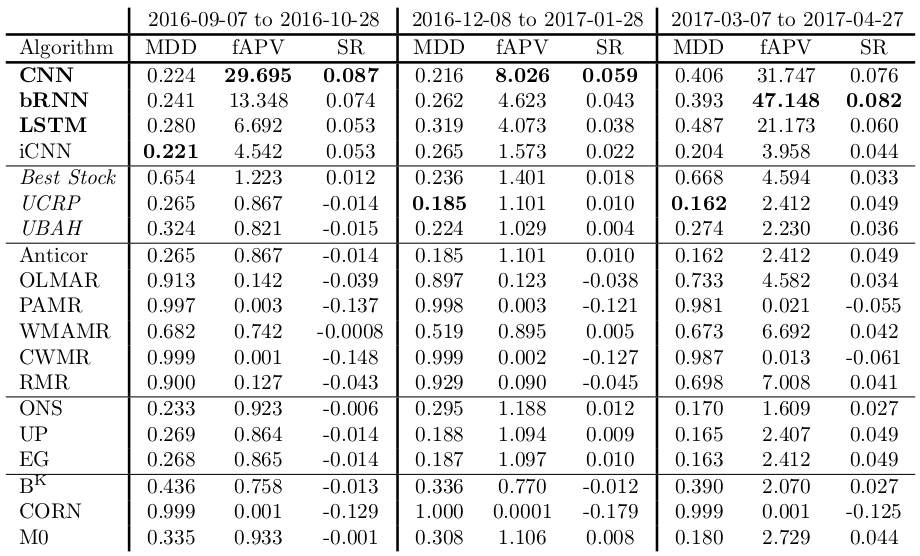
\includegraphics[width=0.55\linewidth]{result.png}
	\caption{Performances of the three EIIE (Ensemble of Identical Independent Evaluators)
		neural networks, an integrated network, and some traditional portfolio selection
		strategies in three different back-test experiments in UTC time on the cryptocurrency exchange Poloniex.}
	\label{fig_result}
\end{figure}

\section{Conclusion and Critique}
This article proposed an extensible reinforcement-learning framework solving the general financial portfolio management problem. Being invented to cope with multi-channel market inputs and directly output portfolio weights as the market actions, the framework can be fit in with different deep neural networks, and is linearly scalable with the portfolio size.
To take transaction cost into account when training the policy networks, the framework
includes a portfolio-weight memory, the PVM, allowing the portfolio-management agent to learn restraining from oversized adjustments between consecutive actions. Finally, the agent was trained using a fully exploiting deterministic policy
gradient method, aiming to maximize the accumulated wealth as the reinforcement reward
function.

The profitability of the framework surpasses all surveyed traditional portfolio-selection Among the three EIIE networks, LSTM had much lower scores than the CNN and the basic RNN. The significant gap in performance between the two RNN species under the same framework might be an indicator to the well-known secret in financial markets, that history repeats itself. Not being designed to forget its input history, a vanilla RNN is more able than a LSTM to exploit repetitive patterns in price movement for higher yields. The gap might also be due to lack of fine-tuning in hyper-parameters for the LSTM.


Despite the success of the EIIE framework in the back-tests, there is room for improvement in future works. The main weakness of the current work is the assumptions of zero market impact and zero slippage. In order to consider market impact and slippage, large
amount of well-documented real-world trading examples will be needed as training data. 
Another shortcoming of the work is that the framework has only been tested in one market. To test its adaptability, the current and
later versions will need to be examined in back-tests and live trading in a more traditional financial market.

In addition, the current award function will have to be amended, if not abandoned, for the reinforcement-learning agent to include awareness of longer-term market reactions. This may be achieved by a critic network.

However, the backbone of the current framework, including the EIIE meta topology, the PVM, and the OSBL scheme,
will continue to take important roles in future versions.

\bibliographystyle{ieeetr}
\begin{thebibliography}{1}
	\bibitem{Jiang2017}	
	[1] Z. Jiang, D. Xu, and J. Liang, “A Deep Reinforcement Learning Framework for the Financial Portfolio Management Problem,” Deep Portf. Manag., 2017.
	
	\bibitem{Ormos2013}
	[2] M. Ormos and A. Urbán, “Performance analysis of log-optimal portfolio strategies with transaction costs,” Quant. Financ., 2013.
	
	\bibitem{Moody2001}
	J. Moody and M. Saffell, “Learning to trade via direct reinforcement,” IEEE Trans. Neural Networks, 2001.
	
	\bibitem{Lo2000}
	A. W. Lo, H. Mamaysky, and J. Wang, “Foundations of technical analysis: Computational algorithms, statistical inference, and empirical implementation,” J. Finance, 2000.
	
	\bibitem{Holt2004}
	C. C. Holt, “Forecasting seasonals and trends by exponentially weighted moving averages,” Int. J. Forecast., 2004.
	
	\bibitem{Sharpe1994}
	W. F. Sharpe, “The Sharpe Ratio,” J. Portf. Manag., 1994.
	
	\bibitem{Magdon2004}
	M. Magdon-Ismail and A. Atiya, “Maximum drawdown,” Risk Mag., 2004.
	
	\bibitem{Jiang2016}
	Z. Jiang and J. Liang, “Cryptocurrency Portfolio Management with Deep Reinforcement Learning,” arXiv, 2016.
	
	\bibitem{Shapira2009}
	Y. Shapira, D. Y. Kenett, E. Ben-Jacob, H. M. Markowitz, G. Bonanno, and N. Vandewalle, “Portfolio Selection: Efficient Diversification of Investments,” Eur. Phys. J. B, 2009.
	
	\bibitem{Li2014}
	B. Li and S. C. H. Hoi, “Online portfolio selection,” ACM Comput. Surv., 2014.
	
	\bibitem{Heaton2017}
	J. B. Heaton, N. G. Polson, and J. H. Witte, “Deep learning for finance: deep portfolios,” Applied Stochastic Models in Business and Industry. 2017.
	
	\bibitem{Freitas2009}
	F. D. Freitas, A. F. De Souza, and A. R. de Almeida, “Prediction-based portfolio optimization model using neural networks,” Neurocomputing, 2009.
	
	\bibitem{Deng2017}
	Y. Deng, F. Bao, Y. Kong, Z. Ren, and Q. Dai, “Deep Direct Reinforcement Learning for Financial Signal Representation and Trading,” IEEE Trans. Neural Networks Learn. Syst., 2017.
	
	\bibitem{Dempster2006}
	M. A. H. Dempster and V. Leemans, “An automated FX trading system using adaptive reinforcement learning,” Expert Syst. Appl., 2006.
	
	\bibitem{Silver2014}
	D. Silver, G. Lever, N. Heess, T. Degris, D. Wierstra, and M. Riedmiller, “Deterministic Policy Gradient Algorithms,” Proc. 31st Int. Conf. Mach. Learn., 2014.
\end{thebibliography}



\end{document}


